\subsection{The echo--antiecho HSQC: gradients and coherence selection}
\label{subsec:theory__hsqc_ea}

\begin{figure}[htbp]
    \centering
    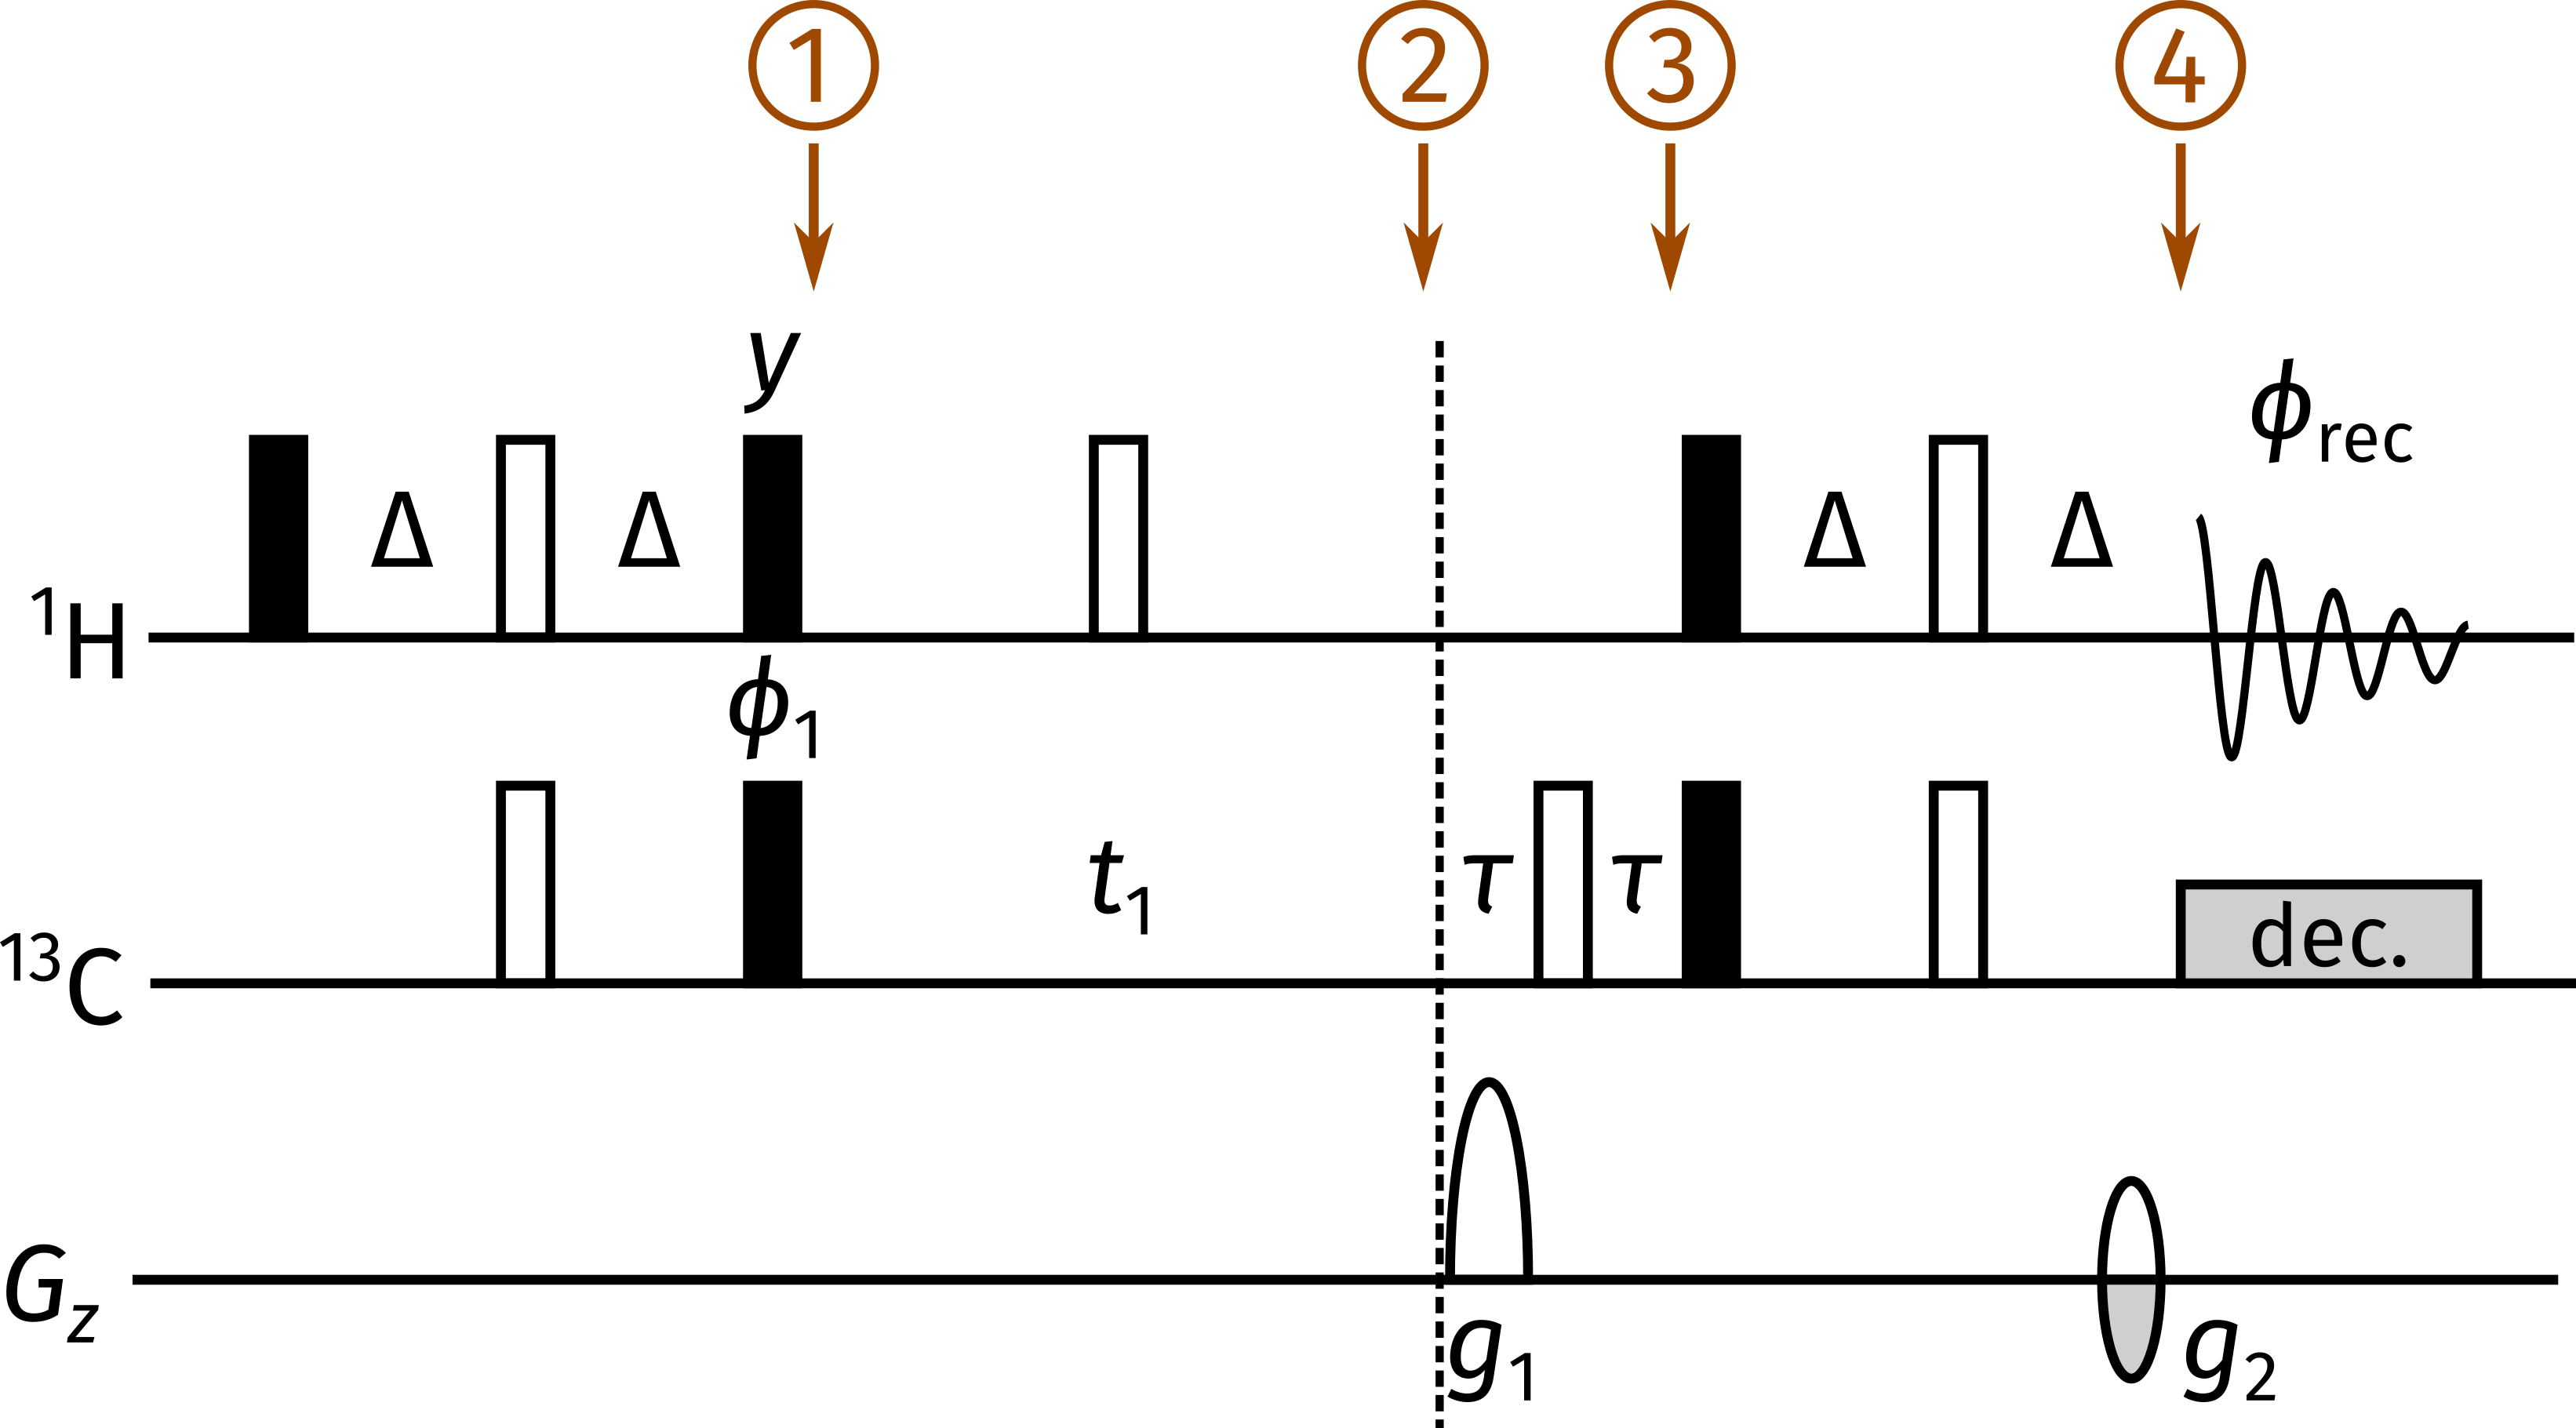
\includegraphics[]{pp/hsqc/etgp.png}%
    \caption[Echo--antiecho HSQC pulse sequence]{
        A typical EA HSQC pulse sequence.
        The delay $\Delta$ is set to $1/(4 \cdot \oneJ{CH})$.
        The gradient amplitudes are chosen such that $|g_1/g_2| = \gamma_{\ch{H}}/\gamma_{\ch{C}} \approx 4$.
        Specifically, the echo dataset is obtained by setting $(g_1, g_2) = (80\%, 20\%)$, and the antiecho dataset by setting $(g_1, g_2) = (80\%, -20\%)$, where gradient amplitudes are quoted as a percentage of the maximum gradient amplitude.
        Unlike in the States HSQC (\cref{fig:hsqc_ph}), phase cycling of $\phi_1$ and $\phi_\text{rec}$ is no longer mandatory as the gradients $g_1$ and $g_2$ dephase unwanted magnetisation.
        $\tau$ represents the duration of both gradients (usually on the order of \SI{1}{ms}).
    }
    \label{fig:hsqc_etgp}
\end{figure}

The EA version of the HSQC experiment (\cref{fig:hsqc_etgp}) is very similar to the States version discussed above.
The only real difference is that two gradients are added: one immediately after $t_1$, and one directly before detection.
As we will see, the effect of this is to enforce a relationship between the coherence orders during the two gradients, or in other words, to select for a specific \textit{coherence transfer pathway} (CTP).

Recall that the Hamiltonian caused by a gradient of strength $G$ is given by $H_\text{grad} = \sum_i \gamma_i Gz I_{iz}$ (\cref{eq:h_grad}), where $z$ is the $z$-position of the spin.
In the case of our two-spin system, we can more explicitly write this as:
\begin{equation}
    \label{eq:h_grad_is_system}
    H_\text{grad} = \gamma_I Gz I_z + \gamma_S Gz S_z.
\end{equation}
Points \circled{1} and \circled{2} are the same as in the States HSQC (\cref{fig:hsqc_ph}), so from \cref{eq:hsqc_ph_after_t1} we know that the density operator at point \circled{2} is:
\begin{equation}
    \label{eq:hsqc_ea_prodop_2}
    \rho = 2I_zS_y\cos(\Omega_S t_1) - 2I_zS_x \sin(\Omega_S t_1).
\end{equation}
In the next spin echo with the gradient $g_1$, $H_\text{offset}$ and $H_\text{J}$ are refocused, so we can ignore their effects.
We assume here that the gradients are applied with duration $\tau$.%
\footnote{In practice, we also need to include a gradient recovery delay immediately after the gradient to allow for the dissipation of eddy currents, which causes the spin echo to be lengthened slightly. This is inconsequential to the analysis and will be ignored here.}
The $I_z$ terms in $\rho$ are unaffected by the gradient since they commute with $H_\text{grad}$; however, the transverse $S$-magnetisation is rotated by a phase which depends on the position of the spin system in the sample.
Immediately after the gradient, we have:
\begin{equation}
    \label{eq:hsqc_ea_gradient}
    \begin{aligned}
        \rho(z) &= 2I_zS_y\cos(\Omega_S t_1)\cos(\gamma_S g_1 z \tau) - 2I_zS_x\cos(\Omega_S t_1)\sin(\gamma_S g_1 z \tau) \\
                &\quad\quad {} - 2I_zS_x \sin(\Omega_S t_1)\cos(\gamma_S g_1 z \tau) - 2I_zS_y\sin(\Omega_S t_1)\sin(\gamma_S g_1 z \tau),
    \end{aligned}
\end{equation}
where the $\rho(z)$ reminds us that this density matrix is spatially dependent.
The $180^\circ_x(S)$ pulse then flips the $S_y$ terms to give us, at point \circled{3},
\begin{equation}
    \label{eq:hsqc_ea_after_grad_echo}
    \begin{aligned}
        \rho(z) &= -2I_zS_y\cos(\Omega_S t_1)\cos(\gamma_S g_1 z \tau) - 2I_zS_x\cos(\Omega_S t_1)\sin(\gamma_S g_1 z \tau) \\
                &\quad\quad {} - 2I_zS_x \sin(\Omega_S t_1)\cos(\gamma_S g_1 z \tau) + 2I_zS_y\sin(\Omega_S t_1)\sin(\gamma_S g_1 z \tau).
    \end{aligned}
\end{equation}
We know already from the States HSQC analysis that the mixing period (i.e.\ reverse INEPT) causes the transformation $2I_zS_y \to I_x$, and that the $2I_zS_x$ term is lost.
So, \textit{if} the gradient $g_2$ were absent, we would have the following terms at point \circled{4}:
\begin{align}
    \label{eq:hsqc_ea_before_g2}
    \rho(z) &= -I_x\cos(\Omega_S t_1)\cos(\gamma_S g_1 z \tau) + I_x\sin(\Omega_S t_1)\sin(\gamma_S g_1 z \tau) \notag \\
            &= -I_x\cos(\Omega_S t_1 + \gamma_S g_1 z\tau).
\end{align}
This is of course not the case.
In principle, the last $\Delta$ delay should be split up into two parts: one of duration $(\Delta - \tau)$ where only $H_{\text{free},I}$ is active, and one of duration $\tau$ where the Hamiltonian $H_\text{free} + H_\text{grad}$ operates.
Thankfully, we know that $H_\text{grad}$ commutes with $H_\text{free,I}$, so we can in fact separate the relevant propagators:
\begin{align}
    \label{eq:propagators_gradient_echo}
    \MoveEqLeft \exp[-\mi(H_{\text{free},I} + H_\text{grad})\tau]\exp[-\mi H_{\text{free},I}(\Delta - \tau)] \notag \\
    &= \exp(-\mi H_\text{grad}\tau) \exp(-\mi H_{\text{free},I}\tau)\exp[-\mi H_{\text{free},I}(\Delta - \tau)] \notag \\
    &= \exp(-\mi H_\text{grad}\tau) \exp(-\mi H_{\text{free},I}\Delta),
\end{align}
where the first (rightmost) propagator is just the delay without a gradient, and the second (leftmost) propagator is just the gradient on its own.
So, we can directly apply $\exp(-\mi H_\text{grad}\tau)$ to the density operator in \cref{eq:hsqc_ea_before_g2} to get:%
\footnote{We have implicitly assumed here that the $z$-coordinate of the $IS$ spin pair during the first gradient is the same as its $z$-coordinate during $g_2$, or in other words, that there is no \textit{diffusion} or \textit{convection} between the two gradients. In general, this is not true, and these effects will lead to a loss of signal as the rephasing by the second gradient is not perfect.}
\begin{align}
    \rho(z) &= -I_x\cos(\Omega_S t_1 + \gamma_S g_1 z \tau)\cos(\gamma_I g_2 z\tau) - I_y\cos(\Omega_S t_1 + \gamma_S g_1 z \tau)\sin(\gamma_I g_2 z\tau) \label{eq:hsqc_ea_after_g2_1} \\
            &= -\frac{1}{2}I_x \cos[\Omega_S t_1 + (\gamma_S g_1 + \gamma_I g_2)z\tau] -\frac{1}{2} I_x \cos[\Omega_S t_1 + (\gamma_S g_1 - \gamma_I g_2) z\tau]  \notag \\
            &\quad\quad - \frac{1}{2}I_y \sin[\Omega_S t_1 + (\gamma_S g_1 + \gamma_I g_2) z\tau] + \frac{1}{2}I_y \sin[\Omega_S t_1 + (\gamma_S g_1 - \gamma_I g_2) z\tau] 
            \label{eq:hsqc_ea_after_g2_2}
\end{align}
(as a sanity check, it can be verified that this reduces to \cref{eq:hsqc_ea_before_g2} if $g_2 = 0$).
The signal which we detect stems from the entire sample length, so we in fact need to perform an integration over $z$:
\begin{equation}
    \label{eq:density_operator_integration}
    \rho = \frac{1}{L} \cdot \int_{-L/2}^{L/2} \rho(z) \,\mathrm{d}z,
\end{equation}
where the sample length is $L$ and $z=0$ is assumed to be the middle of the sample.

For the \textit{echo} experiment, we choose the ratio $g_1/g_2 = \gamma_I/\gamma_S$; this means that $\gamma_S g_1 - \gamma_I g_2 = 0$.
The second and fourth terms in \cref{eq:hsqc_ea_after_g2_2} thus \textit{lose} their $z$-dependence; when integrated over $z$ these terms are unchanged.
On the other hand, the first and third terms are attenuated by a factor proportional to $\int_{-L/2}^{L/2} \cos[(\gamma_S g_1 + \gamma_I g_2)z\tau]\,\mathrm{d}z$ (or equivalently, the sine).
The integrand here can be identified as the phase caused by the evolution under the gradient pulse; we say that the gradients \textit{dephase} coherences. (In the case of the second and fourth terms, they also \textit{rephase} coherences.)
If the gradient strengths $(g_1, g_2)$ and/or their durations $\tau$ are sufficiently large, the integral evaluates to a small number which is effectively zero, corresponding to complete dephasing.
The result is that, just before detection, we have:
\begin{equation}
    \label{eq:hsqc_ea_echo_cartesian}
    \rho = -\frac{1}{2}I_x\cos(\Omega_S t_1) + \frac{1}{2}I_y\sin(\Omega_S t_1),
\end{equation}
or, extracting the detectable $I_-$ components,
\begin{equation}
    \label{eq:hsqc_ea_echo_detectable}
    \rho = -\frac{1}{4}I_-\cos(\Omega_S t_1) + \frac{\mi}{4}I_-\sin(\Omega_S t_1) = -\frac{1}{4}I_-\exp(-\mi\Omega_S t_1).
\end{equation}
Detection of this in $t_2$ gives us the echo signal
\begin{equation}
    \label{eq:hsqc_ea_echo_signal}
    s_\text{echo}(t_1, t_2) = -\frac{1}{4}\exp(\mi \Omega_S t_1)\exp(\mi \Omega_I t_2),
\end{equation}
in accordance with \cref{eq:echo_antiecho_1a}.
Note that the prefactor here is $-1/4$, instead of $1/2$ in the States method (\cref{eq:hsqc_cos_signal,eq:hsqc_sin_signal}): this accounts for the decreased SNR in the EA method as previously described (the minus sign comes from the extra $180^\circ(S)$ pulse after $t_1$, but is inconsequential as it can be removed by phase correction).

In a similar way, it can be shown that if we invert the sign of $g_2$, we have that $g_1/g_2 = -\gamma_I/\gamma_S$.
Now, the second and fourth terms in \cref{eq:hsqc_ea_after_g2_2} are dephased, and we get the antiecho spectrum from this:
\begin{equation}
    \label{eq:hsqc_ea_antiecho_signal}
    s_\text{antiecho}(t_1, t_2) = -\frac{1}{4}\exp(-\mi \Omega_S t_1)\exp(\mi \Omega_I t_2).
\end{equation}

In the above treatment, I have only used the `rules' developed so far for Cartesian product operators to explain the effects of gradients.
\textit{This is clearly very tedious!}
When gradients are involved, it proves simpler to use a different basis, specifically $\{E, I_z, I_+, I_-\}$.
The coherence orders of these, and their products, are easily read off from the terms involved: for example, $I_-S_-$ is double-quantum coherence with $p = -2$.
The evolution of these terms under various Hamiltonians is summarised by Keeler\autocite{Keeler2010}, but two cases are particularly simple and important here:
\begin{enumerate}
    \item $180^\circ_x$ pulses invert $I_z$ and interchange $I_+ \leftrightarrow I_-$;
    \item An operator $I_{ip}$, on a spin $i$ and with coherence order $p$, evolves under the Hamiltonian $\omega I_z$ for a time $t$ to give:
        \begin{equation}
            \label{eq:shift_operator_evolution}
            I_{ip} \longrightarrow I_{ip} \exp(-\mi p\omega t)
        \end{equation}
\end{enumerate}
We have seen examples of the latter before: compare, for example, \cref{eq:rho_coherences,eq:fid_coherences}.
Consider now how a spatially dependent phase is imparted to a coherence as it proceeds through the HSQC sequence.
We assume that between the two gradients the coherence $I_{ip}$ is transferred to $I_{jq}$, i.e.\ $q$-order coherence on some other spin $j$:
\begin{equation}
    \label{eq:shift_operator_evolution_grad}
    I_{ip} \xrightarrow[]{g_1} I_{ip} \exp(-\mi p \gamma_i g_1 z \tau) \xrightarrow[]{\textit{mixing}} I_{jq} \xrightarrow[]{g_2} I_{jq}\exp(-\mi q \gamma_j g_2 z \tau)\exp(-\mi p \gamma_i g_1 z t).
\end{equation}
For the coherence to be rephased, we require that
\begin{equation}
    \label{eq:gradient_refocusing_condition}
    p\gamma_i g_1\tau + q\gamma_j g_2\tau = 0,
\end{equation}
and in the specific case of the HSQC, we know that spins $i$ and $j$ are respectively $S$ and $I$, so
\begin{equation}
    \label{eq:gradient_refocusing_hsqc}
    p\gamma_S g_1 + q\gamma_I g_2 = 0.
\end{equation}
For the echo experiment, we choose $g_1/g_2 = \gamma_I/\gamma_S$, which means that this is satisfied if and only if $p + q = 0$.
Since $I_{q}$ is only detectable if $q = -1$, this means that $p = +1$: in other words, the gradient combination selects for the $I_zS_+$ term during $t_1$.
We also note here that any signal generated from the bulk magnetisation (\proton{} not directly coupled to \carbon{}) cannot be rephased by these gradients: this would require that
\begin{equation}
    \label{eq:unrefocusable_bulk}
    p\gamma_I g_1 + q\gamma_I g_2 = 0 \Leftrightarrow p \gamma_I + q\gamma_S = 0,
\end{equation}
which cannot be satisfied for any sensible integer values of $p$ and $q$ except for $p = q = 0$, which is not observable during $t_2$ anyway.
So, the CTP gradients effectively remove all unwanted signals arising from the bulk magnetisation: the cycling of $\phi_1$ and $\phi_\text{rec}$ done in the States experiment is rendered unnecessary.

Returning to our analysis, at the start of $t_1$ we had the operator $-2I_zS_y = \mi(I_zS_+ - I_zS_-)$.
For the echo experiment, we need only care about the first of these two terms.
This evolves during $t_1$ (and the $180^\circ(I)$ pulse) to give
\begin{equation}
    \label{eq:hsqc_echo_shift_aftert1}
    -\mi I_zS_+ \exp(-\mi \Omega_S t_1).
\end{equation}
The gradient echo after $t_1$ transforms this to
\begin{equation}
    \label{eq:hsqc_echo_shift_after_g1}
    -\mi I_zS_- \exp(-\mi \Omega_S t_1)\exp(-\mi \gamma_S g_1 z\tau) = -\mi I_z(S_x - \mi S_y) \exp(-\mi \Omega_S t_1)\exp(-\mi \gamma_S g_1 z\tau).
\end{equation}
Again, the mixing period only transforms $2I_zS_y \to I_x$, so we get
\begin{equation}
    \label{eq:hsqc_echo_shift_before_g2}
    -\frac{1}{2} I_x \exp(-\mi \Omega_S t_1)\exp(-\mi \gamma_S g_1 z\tau)
\end{equation}
just before applying the $g_2$ gradient.
The $I_x$ term can then be decomposed into $(I_+ + I_-)/2$, and we already know the end of the story: the $I_-$ term is rephased by $g_2$ and then detected to yield $s_\text{echo}(t_1, t_2)$ (\cref{eq:hsqc_ea_echo_signal}).
Being flexible in switching between the two bases can greatly simplify the mathematics involved, as terms which do not survive can be immediately dropped, and the simpler phase modulation $\exp(\mi\omega t)$ can be used instead of unwieldy $\cos(\omega t)$ and $\sin(\omega t)$ terms.

\begin{figure}[htbp]
    \centering
    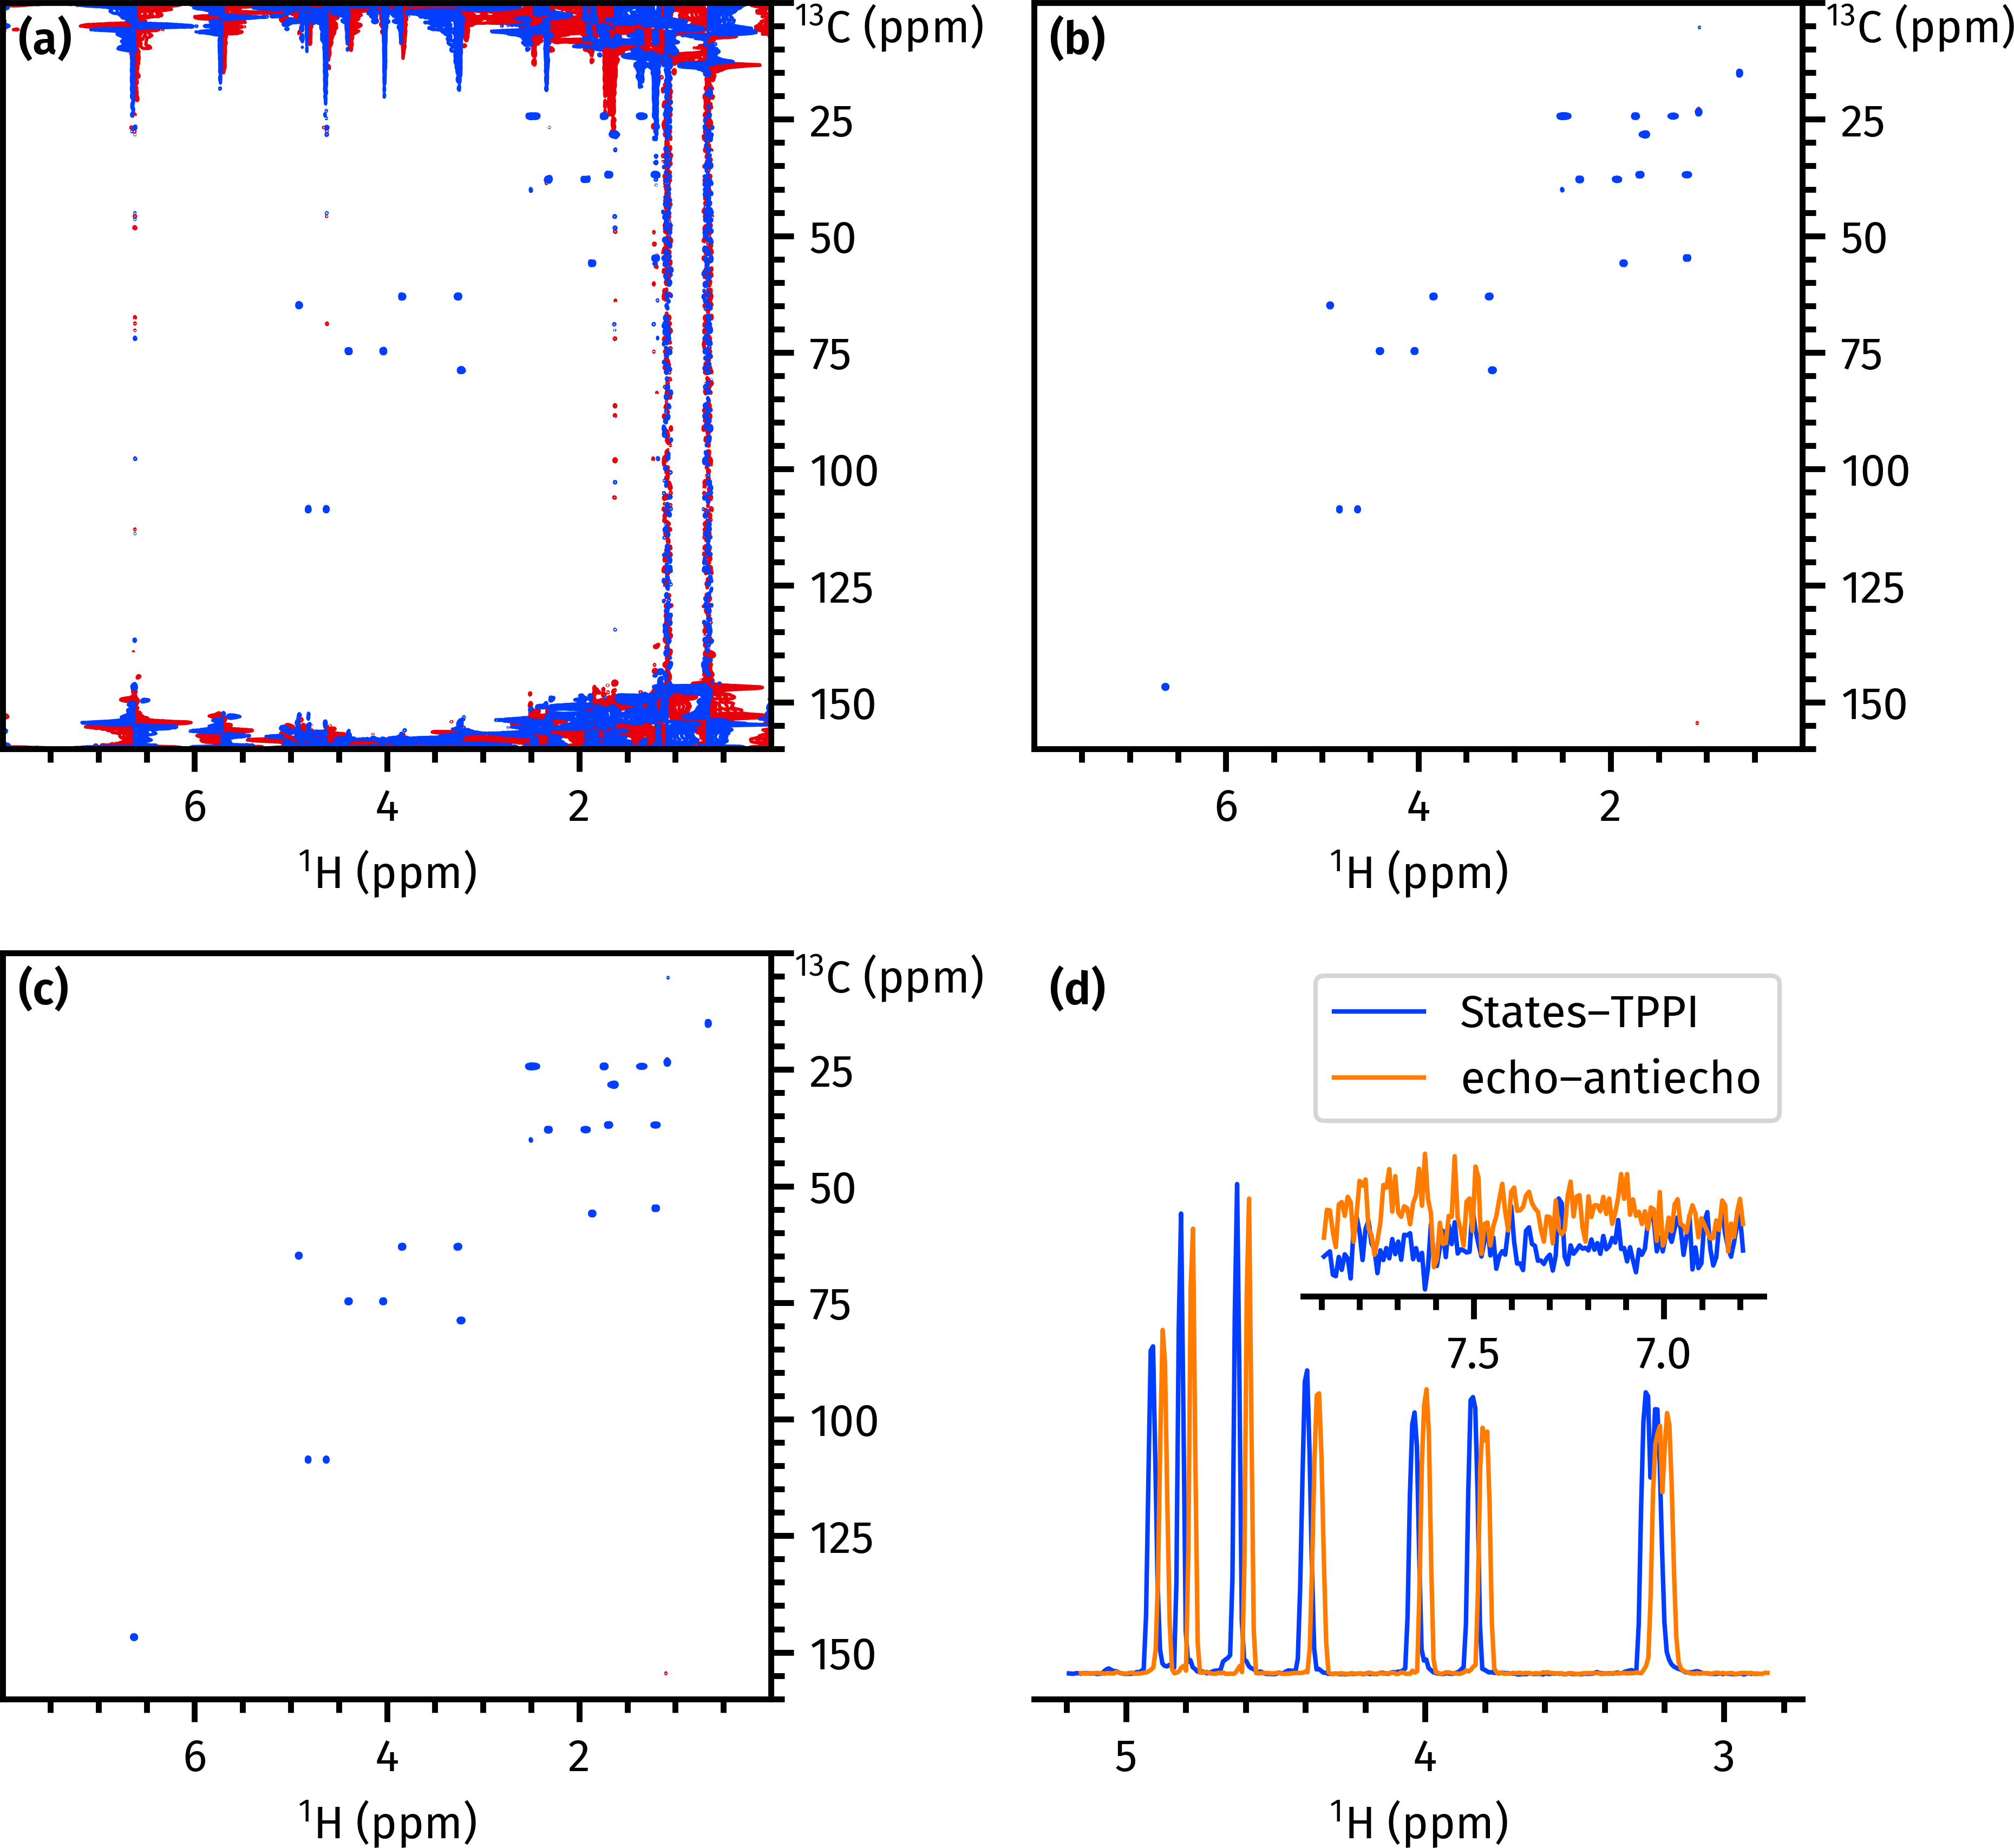
\includegraphics[]{theory/hsqc_comparison.png}%
    {\phantomsubcaption\label{fig:hsqc_comparison_st_ns1}}%
    {\phantomsubcaption\label{fig:hsqc_comparison_ea_ns1}}%
    {\phantomsubcaption\label{fig:hsqc_comparison_st_ns2}}%
    {\phantomsubcaption\label{fig:hsqc_comparison_projections}}%
    \caption[Experimental comparison of States--TPPI and echo--antiecho HSQC]{
        A comparison of HSQC data acquired using various quadrature detection schemes.
        \textbf{(\subref{fig:hsqc_comparison_st_ns1})} States--TPPI HSQC with one scan (i.e.\ no phase cycling) applied.
        \textbf{(\subref{fig:hsqc_comparison_ea_ns1})} EA HSQC with one scan.
        \textbf{(\subref{fig:hsqc_comparison_st_ns2})} States--TPPI HSQC with two scans, using the phase cycling shown in \cref{fig:hsqc_ph}. The artefacts are essentially completely removed.
        \textbf{(\subref{fig:hsqc_comparison_projections})} Projections of the States--TPPI and EA spectra in (\subref{fig:hsqc_comparison_st_ns1}) and (\subref{fig:hsqc_comparison_ea_ns1}) onto the $F_2$ axis (to avoid picking up the artefacts, only the region between 60 and \SI{110}{ppm} in $F_1$ was projected).
        The two projections are slightly horizontally offset for visual clarity.
        The signal intensity is the same, but the noise level in the EA spectrum is larger (by a factor of $\sqrt{2}$, as described in the text).
        \datacode{6A-220809}
    }
    \label{fig:hsqc_comparison}
\end{figure}

The points developed in this chapter are neatly summarised in \cref{fig:hsqc_comparison}.
The States--TPPI experiment (\cref{fig:hsqc_comparison_st_ns1}) is the same as the States experiment in \cref{fig:hsqc_ph}, except that on every $t_1$ increment $\phi_1$ and $\phi_\text{rec}$ are inverted, causing the artefacts to be shifted to the edge of the spectrum.
Comparing the projections of this and the EA experiment (\cref{fig:hsqc_comparison_projections}), it can be seen that the States--TPPI version has a larger SNR by a factor of $\sqrt{2}$; however, it clearly requires at least a two-step phase cycle to obtain presentable data, as was done in \cref{fig:hsqc_comparison_st_ns2}.
Clearly, the sensitivity of the EA spectrum in \cref{fig:hsqc_comparison_ea_ns1} is good enough, rendering the extra SNR from the States--TPPI method unnecessary: it is therefore more practical to use the EA version, as the spectrum quality is much better.
For homonuclear experiments which do not have such stringent artefact suppression requirements, States(--TPPI) quadrature detection is still commonly used.

To end this chapter, we generalise the CTP refocusing requirement introduced in \cref{eq:gradient_refocusing_condition}.
The treatment here is similar to that of Mitschang et al.\autocite{Mitschang1995JCP}
In general, during a pulse sequence we may have $n$ gradients in total, with amplitudes $g^{(1)}, g^{(2)}, \ldots, g^{(n)}$.
We assume that their durations $\tau^{(i)}$ are all the same, such that they can be factored out of the equation.
We express the coherence during the $i$-th gradient as a product of single-spin coherences
\begin{equation}
    \label{eq:generalised_coherence}
    M^{(i)} = \prod_j^{\text{spins}} I_j(p_j^{(i)}),
\end{equation}
where $I_j(p_j^{(i)})$ represents $p_j^{(i)}$-order coherence on spin $j$ during gradient $i$.
The spatially dependent phase imparted by the gradient $g^{(i)}$ is the sum of the phases acquired by each individual coherence:
\begin{equation}
    \label{eq:generalised_phase}
    \phi^{(i)} = -zg^{(i)} \sum_j p_j^{(i)}\gamma_j
\end{equation}
For rephasing of a CTP, we require that $\sum_i \phi^{(i)} = 0$, or equivalently
\begin{equation}
    \label{eq:generalised_rephasing_1}
    \sum_i \left( g^{(i)}\sum_j p_j^{(i)}\gamma_j\right) = 0.
\end{equation}
We can now define a \textit{weighted coherence order}\autocite{John1991JMR} as
\begin{equation}
    \label{eq:weighted_coherence_order}
    p^{(i)} = \sum_j p_j^{(i)}\gamma_j.
\end{equation}
For example, the weighted coherence order for $I_+S_-$ is simply $\gamma_I - \gamma_S$.%
\footnote{Mitschang et al.\ define a \textit{composite coherence order} as $\sum_j p_j^{(i)}\gamma_j/\gamma_I$, using some nuclide $I$ as a reference. This follows an earlier paper\autocite{John1991JMR} where $I$ is explicitly chosen to be \proton{}, and has the advantage that if the experiment is homonuclear (i.e.\ all the spins $j$ are simply $I$), the composite coherence order is the same as the coherence order. Here, I prefer not to tie the analysis to a particular nuclide as the choice of $I$ will likely depend on the experiment under consideration. This different definition naturally induces a different choice of terminology.}
This allows the rephasing condition to be very simply expressed as a scalar product:
\begin{equation}
    \label{eq:generalised_rephasing_2}
    \sum_i g^{(i)} p^{(i)} = \symbf{g} \cdot \symbf{p} = 0.
\end{equation}
$\symbf{g} \cdot \symbf{p}$ can be considered to be an `extent of dephasing': ideally, gradient amplitudes $\symbf{g}$ are chosen such that the desired CTP $\symbf{p}$ is rephased (\cref{eq:generalised_rephasing_2}), and undesired CTPs $\symbf{p'}$ are suppressed as much as possible in that $\symbf{g} \cdot \symbf{p'}$ is maximised.
